\chapter{Methodologies}
\label{chap:methods}
\glsreset{rl}
\glsreset{il}

This chapter illustrates the methodology used to approach the development 
process of this work. 
We start Section \ref{sec:MAS} by analysing the domain of the problem and then 
defining in Section \ref{sec:imitlrng} the learning method.
We continue with a presentation of the approaches considered in Section 
\ref{sec:approaches}, followed by Section \ref{sec:dataset} that describes the type 
of data used for this purpose and how they are generated.
We conclude Section \ref{sec:controllersmodel} with a detailed explanation of the 
controllers used and of the models implemented. 


\section{Multi-agent system}
\label{sec:MAS}

In this work, we investigate collaborative scenarios in a homogeneous \gls{mas}.

In a given simulated \gls{1d} environment, we consider a team of $N$ interacting 
agents, that are assumed to be interchangeable since they have the same physical 
structure and observation capabilities, which collaborate to solve a given common 
goal \cite[][]{stone2000multiagent, vsovsic2016inverse}.

This system, containing agents also called ``swarming agents’’, in principle is an 
extension of a \gls{decpomdp} \cite[][]{oliehoek2012decentralised}, and can be 
formally defined as a tuple $(S, O, A, R, \pi)$, \cite[][]{schaal1999imitation}, 
where:
\begin{itemize}
	\item $S$ is the state of the system, or the set of local states for each agent, 
	composed of all the possible combinations of positions and observations.
	\item $O$ is the set of possible observations for each agent, obtained through 
	the sensors.
	\item $A$ is the set of possible actions for each agent.
	\item $R$ is the reward function $S \times A \rightarrow \mathbb{R}$.
	\item $\pi$ is the policy $S \rightarrow A$ which determines the action to 
	execute in a given state for every single agent.
\end{itemize}

As introduced in Chapter \hyperref[chap:intro]{Introduction}, through the course 
of this study we tackle two \gls{ma} scenarios. In both of them, the agents have a 
common goal that requires them to cooperate to achieve it. 

Three popular approaches used to solve cooperative \gls{ma} problems are 
Supervised and Unsupervised learning, and \gls{rl}, which are distinguished 
according to the type of feedback provided to the agent: the target output in the 
first case, no feedback is provided in the second, and reward based on the learned 
output in the last one \cite[][]{panait2005cooperative}.
However, in reward-based methods, it is notoriously hard to design a suitable 
reward function, able to lead to the desired behaviour in all possible scenarios, 
even for complex tasks \cite[][]{hadfield2017inverse}.
\gls{il} methods can be used to overcome this problem by learning a policy from 
expert demonstrations without access to a reward signal \cite[][]{song2018multi}.

\section{Imitation learning}
\label{sec:imitlrng}
\glsreset{rl}
\glsreset{il}
\glsreset{nn}

\gls{il} is a class of methods that has been successfully applied to a wide range of 
domains in robotics, for example, autonomous driving.
Unlike reward-based methods, \gls{il} acquires skills by directly observing 
demonstrations of the desired behaviour in order to provide a learning signal to 
the agents \cite[][]{zhang2018deep}.

A typical approach to \gls{il}, also called Behavioural Cloning 
\cite[][]{torabi2018behavioral}, is a supervised technique that consists in 
collecting a certain amount of data, corresponding to a sequence of encountered 
observations and actions performed by a teacher agent which acts according to 
an unknown policy in order to achieve a certain goal.
Then, the demonstrations of the expert’s behaviour are used to learn a controller, 
by training usually a classifier or regressor, that predict behaviour to correctly 
achieve the same goal in a certain environment \cite[][]{ross2011reduction}.
The machine learning model should be able to learn how to extract relevant 
information from the data provided to it, directly learning a mapping from 
observations to actions.

Instead, an unsupervised approach collects only the data that correspond to a 
sequence of encountered observations performed by a teacher agent, and the 
learned controller should be able to infer the correspondence from observations 
to actions and find a way to accomplish the same task \cite[][]{stadie2017third}.
In this case, learning a good model is more challenging since the coordination, 
that is implicit in the demonstrations, has to be inferred as a latent variable 
\cite[][]{le2017coordinated}.

\section{Approaches}
\label{sec:approaches}
Given the two scenarios presented in Chapter \hyperref[chap:intro]{Introduction}, 
distributing the robots in space such that they stand at equal distance from each 
other and colouring the robots in space depending depending on their position 
with respect to the others in the group, through the course of this study we tackle 
two \gls{ma} scenarios. In both of them, the agents have a common goal that 
requires them to cooperate to achieve it. 

While both are excellent examples of distributed tasks, they have an important 
difference: the first problem can be solved without using communication, while 
for the second one it is necessary.
A full explanation of how communication works for Thymio II is covered in 
Section \ref{subsec:thymiocomm}.

\subsection{Distributed approach}
\label{subsec:dist}

As stated before, the first task can be accomplished with a distributed approach 
without communication.
The agents share the same goal: arrange themselves uniformly along the line 
between the two “dead” robots, in such a way they stand at equal distances from 
each other.
This problem represents an example of a cooperative task, for this reason, it will 
be desirable for the agents to cooperate \cite[][]{barrett2017making}. 

On the one hand, when communication is not possible, they can achieve their 
goal without directly interact with each other. 
As stated by Holland in \emph{Multiagent systems: Lessons from social insects and 
collective robotics} \cite[][]{holland1996multiagent}, since the agents exist in the 
same environment, they can affect each other indirectly in several ways.
For instance, they can be sensed from the other robot’s or they can even change 
the state of an agent by applying a force on it, for example, by colliding with it.
The work of Grassè about Stigmergy Theory provides additional details about 
active and passive stigmergy \cite[][]{grasse1959reconstruction}.

On the other hand, the difficulty of the problem we consider is that the agent 
does not have full knowledge of its mates’ behaviours.
Although a communication protocol is not necessary, allowing an explicit 
exchange of messages between the agents may nonetheless increase agent 
performance: they use the exchange of message in order to coordinate more 
effectively and distribute more accurately, finally reaching a more efficient 
solution \cite[][]{panait2005cooperative}.

\subsection{Distributed approach with communication}
\label{subsec:comm}
In the second task also, the agents share a common goal: assuming that they are 
divided into groups, which are unknown to them, their objective is to determine  
their group membership and to colour themselves accordingly. 
For this kind of problems, allow explicit communication is not a plus but a 
necessity.

An important aspect that needs to be considered is the decision of what to 
communicate and when, so that no issues arise.

Regarding the communication content, the agents can, for example, inform the 
others of their current state by sharing the sensor readings, or even information 
about the past \cite[][]{guestrin2002coordinated, panait2005cooperative}.
For this purpose, we used an unsupervised approach in which we do not have to 
specify the communication content, which instead has to be inferred by the 
network as a latent variable.

Of great importance is also the moment in which transmit a message. In fact, if the 
communication is delayed, it can become useless or even cause unwanted 
behaviour \cite[][]{stone2000multiagent}.
As we have already said in Section \ref{subsec:thymiocomm}, each robot transmits 
a message every $0.1$\gls{s} and likewise receives one for each of the sensors. In 
our case, we expect each agent to receive two communications, one from each of 
its respective neighbours. With real robots, but also in simulation, what we want to 
attain is a synchronous communication update protocol. Formally, each robot 
$n$, given the observations at time $t$, that corresponds to the sensor readings 
$S_n(t)$, and the communications at time $t-1$, in particular $C_{n-1}(t-1)$ 
and $C_{n+1}(t-1)$, calculates the control $V_n(t)$ and the message to 
transmit $C_n(t)$ at time $t$. 
Adopting this technique, it is not important to keep track of the order of the 
robots and it is as if the agents operate simultaneously. 
Ideally, the frequency of updates must be lower than that with which the 
robots exchange messages, however, it can happen that due to delays or 
noise in the sensor readings the communication of some robots is not 
received or transmitted. In this case, the array is not updated and the last 
received message is kept instead, without causing undesired behaviour but simply 
a slowdown.

\section{Data collection}
\label{sec:dataset}

In this work, $N$ robots, all oriented in the same direction, are initially 
randomly placed along the $x$-axis, avoiding collisions and in such a way the 
average gap among them is included in the proximity sensors' ranges. 
All agents act in collaboration to achieve a common goal, except the first and last 
in the row that behave like walls.

Each robot can be considered as a point on the plane, formally described by a 
homogeneous vector with respect to the world coordinate frame $W$, obtained 
multiplying the homogeneous vector of the point \gls{wrt} the robot coordinate 
frame $A$, by a homogeneous transformation. The relative pose $A$ of each 
agent is identified by a $3 \times 3$ matrix $\mathbf{T}$, with respect to the 
world reference frame $W$. 
\begin{Equation}[!htb]
	\centering
	\begin{equation}
	{^W\!\xi_A} = {^W\!\mathbf{T}_A} 
	=
	\begin{pmatrix}
	^W\!\mathbf{R}_A & ^W\!\mathbf{t}_A\\
	0, 0 & 1
	\end{pmatrix}
	=
	\begin{pmatrix}
	\cos \theta & - \sin \theta & t_x\\
	\sin \theta & \cos \theta & t_y\\
	0 & 0 & 1
	\end{pmatrix}
	\end{equation}
	\caption[Homogeneous transformation matrix.]{The homogeneous 
		transformation matrix, 	$^W\!\mathbf{T}_A$, includes $^W\!\mathbf{R}_A$, 
		a 
		$2 \times 2$ rotation matrix and $^W\!\mathbf{t}_A$, a $2 \times 1$ 
		translation vector.}
	\label{eq:hommatrix}
\end{Equation}
However, since they are arranged on a line, the environment can be considered 
\gls{1d}, hence, the $y$ coordinate is equal to $0$ and also the orientation angle 
$\theta$ must be zero as all the agents are oriented as the world frame. 
Moreover, we can consider the agents as holonomic, since their movements are 
limited to only one dimension. This premise simplifies our system, in which 
consequently we have to keep into account only geometric constraints and not
kinematic.

Of fundamental importance is the approach adopted for the generation of the 
starting positions of the robots.
The initial configurations need to be randomly generated, verifying that there is 
no bias towards those close to the target.
In particular, once established the number of agents to spawn and the average 
gap between them, a vector containing samples, each representing a random 
gap in $\mathbb{R}$, is drawn from a uniform distribution in the interval $[0, 
2*\mathtt{avg\_gap})$. 
The length of the Thymio, that is $10.9$ \gls{cm}, is added to each gap, then the 
final positions are obtained by returning the cumulative sum of the elements in 
the generated vector. 

Another premise regards the sensors of the Thymio: as introduced in Section 
\ref{subsec:enkisensors}, we have available \texttt{prox\_values} and 
\texttt{prox\_comm\_events.intensities}. Before being used, the 
\texttt{prox\_comm\_events.intensities} should be flattened to obtain a single 
array containing the intensities of all recorded events. 
To do so, we decided to create a new array, called \texttt{prox\_comm}, by 
keeping for each element only the value with the maximum intensity among the 
possible values in the corresponding position of the original vectors – for this 
purpose maximum $2$.
In addition, we define another variable, named \texttt{all\_sensors}, which is an 
array of $14$ intensities resulting from the combination of the 
\texttt{prox\_values} and \texttt{prox\_comm} vectors.

The data that we use to train our machine learning models are generated through 
Enki, the simulator introduced in Section \ref{sec:enki}.
In particular, two datasets containing $1000$ simulation runs each are built using 
the omniscient and the manual controllers, that will be explained in Sections 
\ref{subsec:expert} and \ref{subsec:manual}. 
Each run, that differs from the others for the initial positions of the agents, sets up 
a world containing $N$ Thymio. 
In particular, for all the simulations the number of agents $N$ is chosen randomly 
within the range $[5, 10]$, and the \texttt{avg\_gap}, that is the average distance 
among the robot in the final configuration of the run, that can be in the range 
$[5, 24]$.
A simulation run is stopped either immediately after all the robots reach the 
target pose, with a certain tolerance, or after $4$\gls{s} ($40$ time steps).
At each time step, all the useful information regarding the agents is stored in 
the dataset, such as the sensor readings, the pose of the robot, the motors target, 
the communication transmitted and received and its colour.

All the original datasets are shuffled, based on the single run, in order to improve 
the generalisation on the samples, and then split the resulting collection into 
train, validation and test sets, containing respectively 60-20-20\% of the data.
The dataset generated using the expert controller is the one used to train the 
networks, while the one generated with the manual controller is used as a 
baseline for the comparison with the learned model.

\section{Controllers}
\label{sec:controllersmodel}

\glsreset{il}
\glsreset{mas}

In a \gls{mas}, each agent can perceive the environment through sensors 
acquiring a total or partial knowledge of it. The observations can be used by a 
controller, the key component of the system introduced in Section 
\ref{subsec:control}, together with the current state of the agents, to determine 
actions, draw inferences and finally solve tasks. 

For the two scenarios that we consider in this study, the state of the agent is the 
combination of four elements: its position on the $x$-axis, the observations, i.e. 
the distances from neighbours recorded in the sensor readings, communication 
messages, one transmitted to the two nearest neighbours, one on the left and the 
other on the right, and two received from peer robots, and finally its colour.
Instead, the set of actions that agents can perform are different depending on 
the task: in the first scenario the agents move forward and backwards along the 
x-axis, therefore the set includes the range of velocity that they can assume; in the 
second one, the agents  can turn on their top RGB LED in red or blu, so the set this 
time is composed by the two possible colours.

In an \gls{il} setting, there are two main controllers involved: an omniscient 
controller, which decide the best action exploiting its perfect knowledge of the 
state of the system, and a learned controller, which imitate the behaviour of the 
expert.
Undoubtedly, one of the main advantages of adopting a \gls{ml} model to solve 
these tasks is that the algorithm must learn how to extract relevant information 
from the data it receives, sidestepping the difficulty of manually implementing the 
perception part.
However, for the tasks that we are going to face, we introduce three controllers: in 
addition to the two mentioned before, we also use a manual controller, which can 
observe only parts of the system. As a consequence, its decisions do not depend 
on the state of the whole swarm \cite[][]{vsovsic2016inverse}.

\subsection{Expert controller}
\label{subsec:expert}

As just described, the first element involved in an imitation learning problem is 
the omniscient controller, also called expert. 
This is a centralised controller that perceives the environment and observes the 
state and the observations of all agents, obtaining a global knowledge of the state 
of the system. In this way, it can use all the information to decide the best action 
to perform for all the agents. 

As the goals to be achieved vary, the controllers should act differently. For this 
reason, in the following paragraphs we define the approaches used for the 
implementation of the controllers in the two scenarios.

\subsubsection{Task 1: Distributing the robots in space}
\label{subsubsec:experttask1}

In the first scenario, the omniscient controller, based on the current poses of the 
robots, moves the agents at a certain speed to reach the target positions. In 
particular, the linear velocity of each agent is computed as a ``signed distance`` 
between the current and the goal position of the robot, along its theta. 

Formally, given the current pose, defined by the triple $(x, y, \theta)$ and the 
target pose $(\overline x, \overline y, \overline \theta)$, the signed distance $d$ 
is computed as follow:
\begin{Equation}[!htb]
	\centering
	\begin{equation}
	d = \left(\overline x * \cos (\theta) + \overline y * \sin (\theta)\right) -
	\left( x * \cos (\theta) + y * \sin (\theta)\right)
	\end{equation}
	\caption[Signed distance function.]{Function used to compute the ``signed 
		distance'' between the current and the goal position of a robot.}
	\label{eq:signeddist}
\end{Equation}

\noindent
To obtain the final velocity of the agent, this quantity is multiplied by a constant, 
we choose $10$ to keep the controller as fast as possible, and then clipped to the 
maximum value supported by Thymio II, $16.6$\gls{cm/s}.

This controller can be considered as a variant of a Bang Bang controller, 
introduced in Section \ref{subsubsec:bangbang}, since the optimal controller 
moves the robot at maximum speed towards the target unless the target is closer 
than \texttt{control\_step\_duration} $\times$ \texttt{maximum\_speed}. In this 
case, the agent is moved slower than maximum speed so that at the end of the 
time step it is located exactly at the target.

\subsubsection{Task 2: Colouring the robots in space}
%FIXME
In this scenario, the omniscient controller, based on the current poses of each 
robot, is able to determine the order of the agents and turn on their top \gls{led}  
in one time step. For this reason, we decided to use the same dataset obtained for 
the previous task, but adding to it the colour of the robot, in order to provide the 
network with examples consisting of multiple time steps from which it can learn.


\subsection{Manual controller}
\label{subsec:manual}

Unfortunately, centralised solutions for distributed problems are not feasible in 
real situations since agents do not have access to their states but only to their local 
observations. The global state of the system, accessible to a centralised controller, 
in this case, is hidden from each agent who therefore cannot understand its 
absolute position.
Instead, we are interested in situations in which is used a local controller to decide 
the next action, based on the individual agent's observations, or even cases in 
which the programming part of the controller is automated.
In fact, the main purpose of this controller is to draw conclusions about the 
quality of the controller learned.

As before, to different goals to be achieved correspond different controllers 
that should act differently. For this reason, in the following paragraphs we define 
the approaches used for the implementation of the controllers in the two 
scenarios.

\subsubsection{Task 1: Distributing the robots in space}
\label{subsubsec:manualtask1}
\glsreset{pid}
In the first scenario, the controller is in charge of moving the robots towards the 
target by minimising the difference between the values recorded by the front and 
rear sensors, trying to maintain the maximum achievable speed.

For each agent, the controller is the same and, if given an identical set of 
observations as input, likewise, the outputs will be equivalent.

The kind of controller we decided to implement for this purpose is a Proportional 
(P) controller, a particular variant of the \gls{pid} controller with only the $K_p$ 
term, described in detail in Section \ref{subsubsec:pid}. 
In particular, the value of the proportional gain has been tuned to yield 
satisfactory performance so that the system is stable, as shown in Figure 
\ref{fig:pid}. 

\begin{figure}[htb]
	\centering
	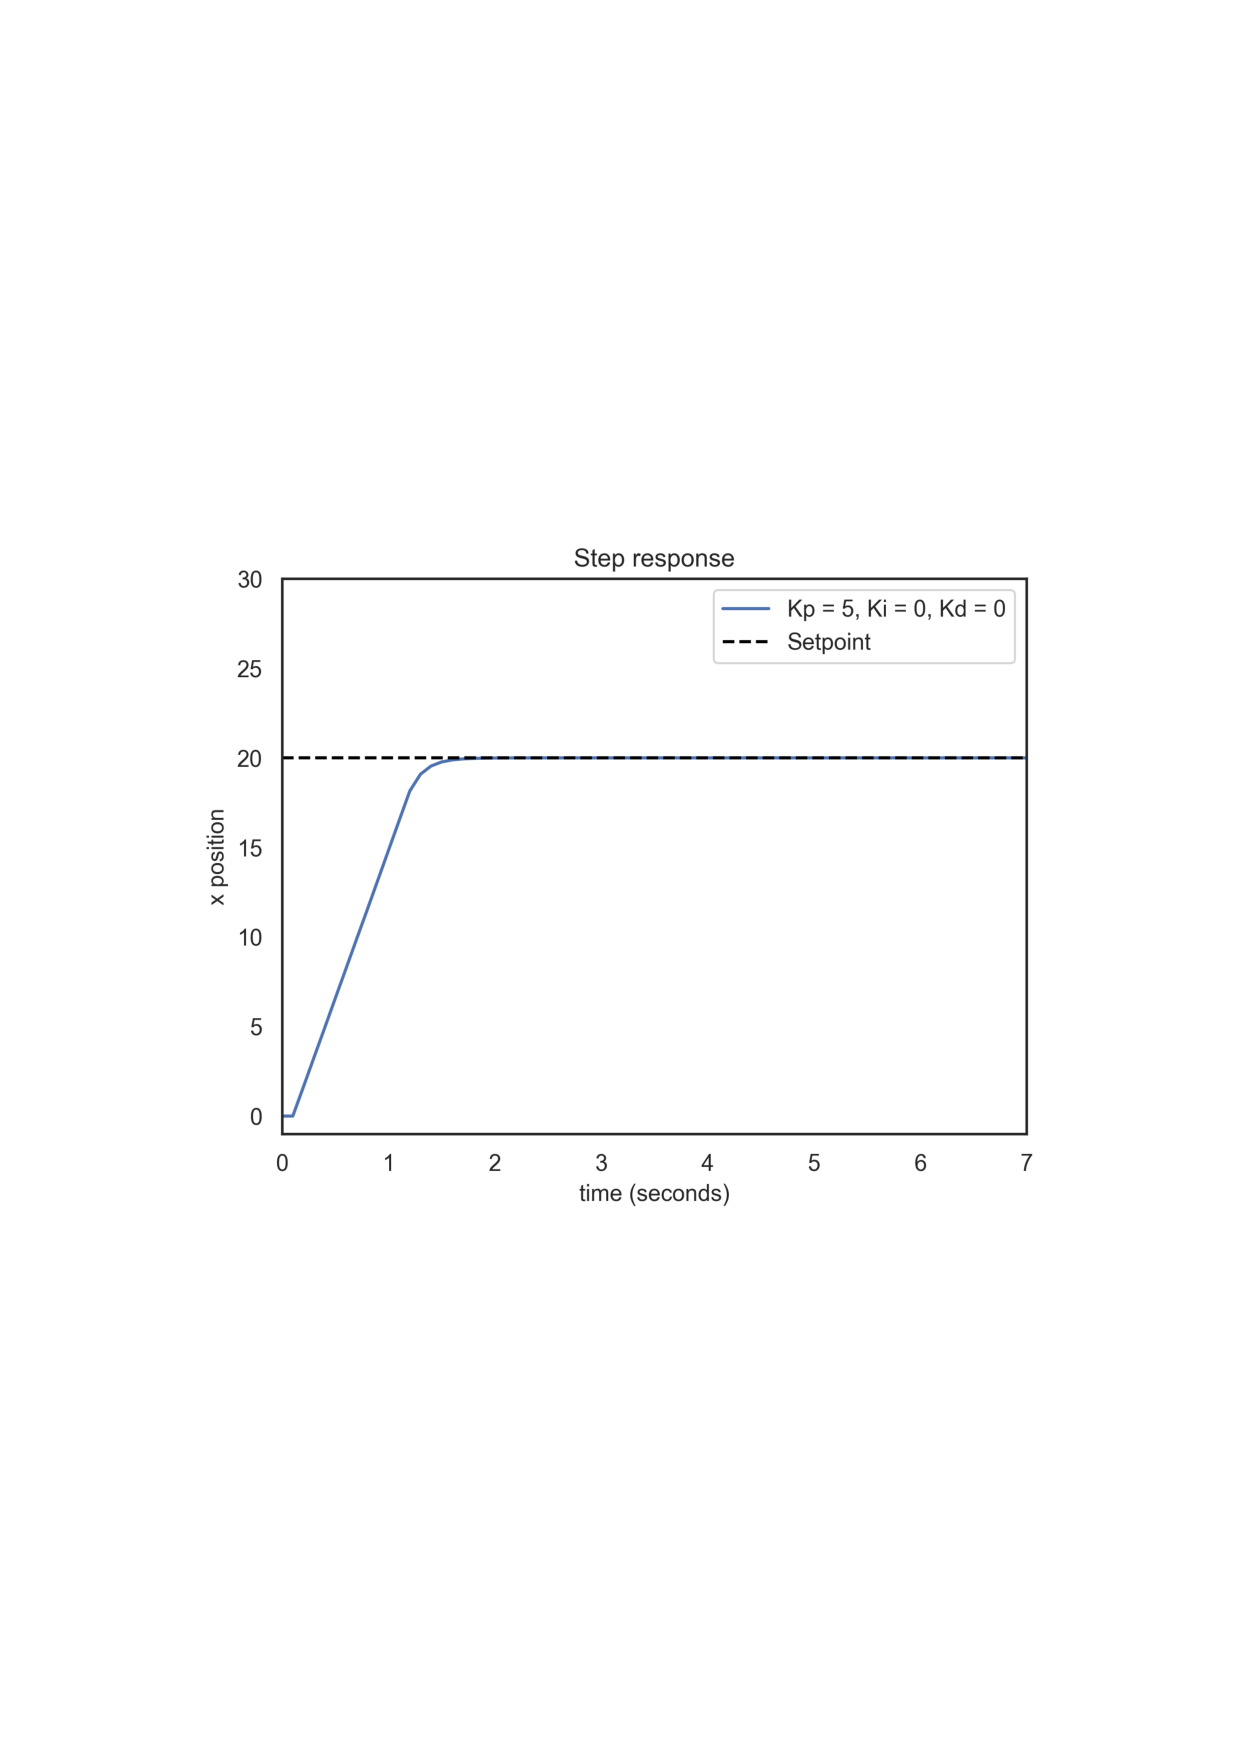
\includegraphics[width=.5\textwidth]{contents/images/Step-responsep=kp5ki0kd0}
	\caption[Step response of the proportinal PID controller.]{Visualisation of the 
		step-response of a P controller with proportional 
		gain $5$.}
	\label{fig:pid}
\end{figure}

It is important to notice that the speed returned by the controller is used to set the 
\texttt{motor\_\{left, right\}\_target}, both with the same value, in order to move 
the robots straight ahead. Moreover, the first and the last robots of the line, 
whose sensors never receive a response respectively from the back and from the 
front, never move.

\subsubsection{Task 2: Colouring the robots in space}
In this scenario, the robots observations, in particular, the sensor readings, do not 
provide useful information about the order of the agents, therefore they are not 
considered to accomplish this task.
On the other hand, if an omniscient controller is not employed, it is impossible to 
solve the problem without using communication, since it is the only way for the 
agents to understand their ordering.

Thus, by initially making all robots transmit the same value, i.e. $0$, we are able 
to establish which are the first and the last robots in the row, or those that do not 
receive any communication respectively from back and front. 
These two agents can at this point start the actual communication by transmitting 
the value they received, increased by $1$, that is $1$. 
The following robots will in turn transmit the value they have received, increased 
by one. Since the messages received by each of them are two, the agents will in a 
sense, learn to count in order to understand which is the correct value to 
transmit.

The protocol used to decide the communication and the colour, which also 
depends on the amount of robots $N$, or if there are even or odd numbers, is 
shown in Listing \ref{lst:manualtask2}. The colour of each agent in the initial 
configuration is randomly chosen between the two possible colours, red and blue.

\medskip
\begin{python}
	c_left, c_right = get_received_communication(state)
	
	if N % 2 == 1:  # if the number of robots is odd
	
	# Case 1: no communication received from left
	if c_left == 0:
	if c_right > N // 2:
	# the agent is in the first half of the row, so its colour is blue
	message = c_right - 1
	colour = 1
	elif c_right == N // 2:
	# the agent is the central one, so its colour is blue
	message = c_right + 1
	colour = 1
	else:
	# the agent is in the second half of the row, so its colour is red
	message = c_right + 1
	colour = 0
	
	# Case 2: no communication received from right
	elif c_right == 0:
	if c_left > N // 2:
	# the agent is in the second half of the row, so its colour is red
	message = c_left - 1
	colour = 0
	elif c_left == N // 2:
	# the agent is the central one, so its colour is blue
	message = c_left + 1
	colour = 1
	else:
	# the agent is in the first half of the row, so its colour is blue
	message = c_left+ 1
	colour = 1
	
	# Case 3: communication received from both sides
	else:
	if c_left > c_right:
	# the agent is in the second half of the row, so its colour is red
	message = c_right + 1
	colour = 0
	else:
	# the agent is in the first half of the row, so its colour is blue
	message = c_left + 1
	colour = 1
	
	
	elif self.N % 2 == 0:  # if the number of robots is even
	
	# Case 1: no communication received from left
	if c_left == 0:
	if c_right > N // 2:
	# the agent is in the first half of the row, so its colour is blue
	# the situation is ambiguous the message to transmit could be c_right or 
	# even c_right - 1
	message = c_right
	colour = 1
	else:
	# the agent is in the second half of the row, so its colour is red
	message = c_right + 1
	colour = 0
	
	# Case 2: no communication received from right
	elif c_right == 0:
	if c_left < N // 2:
	# the agent is in the first half of the row, so its colour is blue
	message = c_left + 1
	colour = 1
	else:
	# the agent is in the second half of the row, so its colour is red
	# the situation is ambiguous the message to transmit could be c_left or 
	# even c_left - 1
	message = c_left
	colour = 0
	
	# Case 3: communication received from both sides
	else:
	if c_left > c_right:
	# the agent is in the second half of the row, so its colour is red
	message = c_right + 1
	colour = 0
	elif c_left < c_right:
	# the agent is in the first half of the row, so its colour is blue
	message = c_left + 1
	colour = 1
	else:
	# the agent is in the second half of the row, so its colour is red
	message = c_left
	colour = 0
\end{python}

\begin{lstlisting}[frame=none,caption=Protocol used from the manual controller 
to decide for each robot the message to transmit and the colour., 
label=lst:manualtask2]
\end{lstlisting}


\subsection{Learned controller}
\label{subsec:learned}

Usually, to train a network that learns a controller, the states and the actions, 
provided by an expert, need to be observable. For this study, we have decided to 
use the observations of the robots instead of the state, i.e. the positions. 
The reason behind this decision is that in most environments, agents are never 
actually exposed to the full state of this system. Instead, they receive partial 
observations, often local or incomplete. In addition, it is frequently too expensive 
to provide the agent with the full state of the system, and sometimes it is not even 
clear how to represent it \cite[][]{ml-agents}.

As the goals to be achieved vary, the controllers should act differently. For this 
reason, we define distinct approaches for the implementation of the controllers 
in the two scenarios.
Regarding the first task, we consider two different networks: one distributed that 
act in a supervised way, and one that, in addition to predicting the control output, 
infers a communication protocol between the agents. 
In the second task, we trained one network that predicts the colour output and in 
addition, as before, infers the communication between the robots.

\subsubsection{Task 1: Distributing the robots in space without using 
communication}

Using the data collected through the simulator using the expert controller, it is 
possible to train a very simple ``distributed network'' that takes as input an array 
containing the response values of the sensors – which can be either 
\texttt{prox\_values}, \texttt{prox\_comm} or \texttt{all\_sensors} – and produces 
as output an array containing one float that represents the speed of the wheels, 
which is assumed to be the same both right and left.

The training dataset then contains a fixed number of simulation runs, each 
composed of a variable quantity of time steps. It is important to notice that 
for this approach, unlike the one with communication, it is neither necessary to 
preserve the order of the sequence of time steps, nor to know the exact number 
of agents in the simulation since the network input is the sensing of a single robot.

For this reason, the model is independent of the number of agents and 
consequently it is possible to prove its generalisation capacity, regardless the 
number of robots, by training the networks first on datasets each with a different 
but fixed value of $N$ and then evaluating them on simulations with a variable 
$N$.
It is easy to show that, although the value of $N$ changes, the network structure 
does not, as it is sufficient during the input preprocessing to change the 
dimension of the input in such a way that all the tensors have the same length, 
fixed at the maximum possible value of $N$, padding those tensors with a lower 
number of agents.

The architecture of the network, displayed in Figure 
\ref{fig:singlenetdistributed1}, is straightforward: there are three linear layers of 
size $\langle\mathtt{input\_size}, 10\rangle$,  $\langle 10, 
10\rangle$ and $\langle 10, 1\rangle$, where \texttt{input\_size} is the 
shape of the sensing that can be either $7$ or $14$.
\begin{figure}[htb]
	\centering
	\begin{subfigure}[h]{0.495\textwidth}
		\centering
		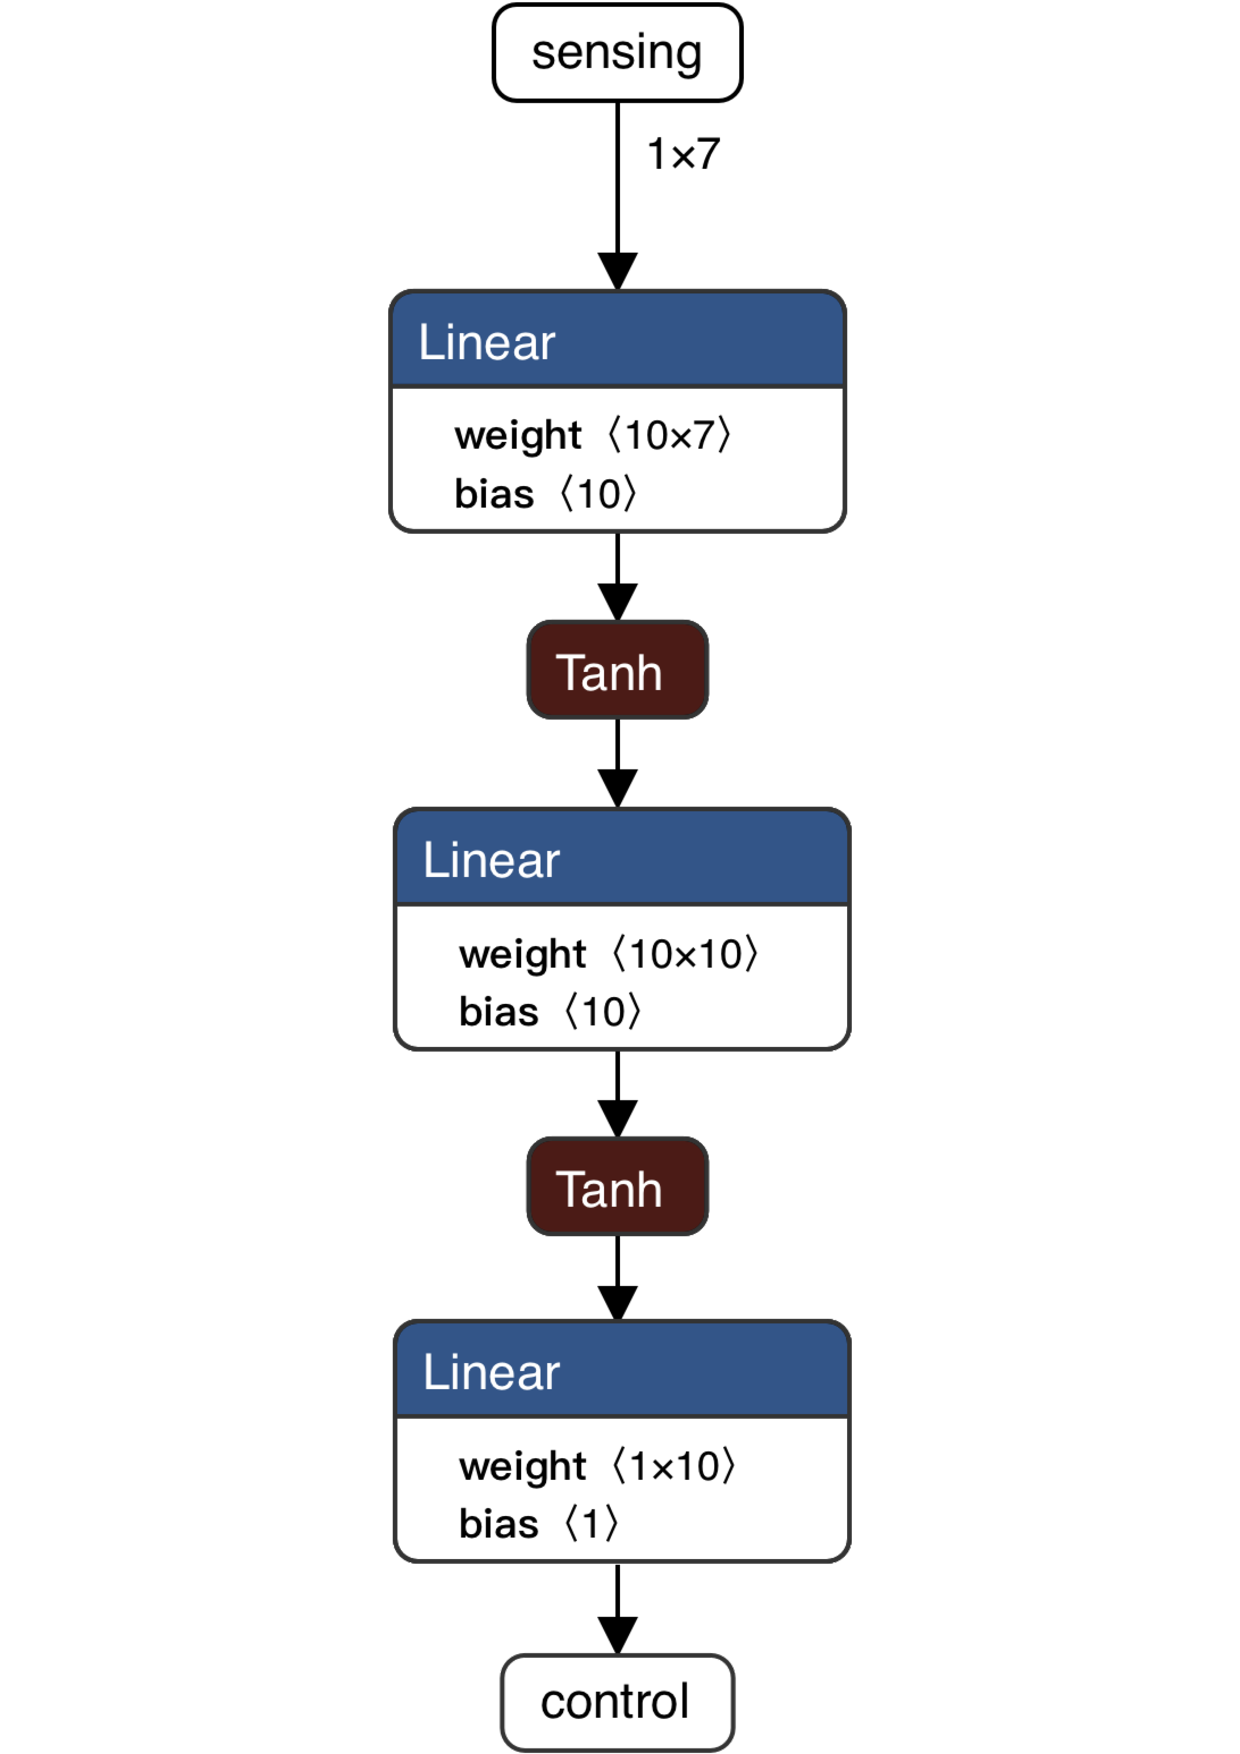
\includegraphics[width=.8\textwidth]{contents/images/task1distributed@4x}%
		\caption{Network with $7$ input sensing.}
		\label{fig:singlenet-d7distributed1}
	\end{subfigure}
	\hfill
	\begin{subfigure}[h]{0.495\textwidth}
		\centering
		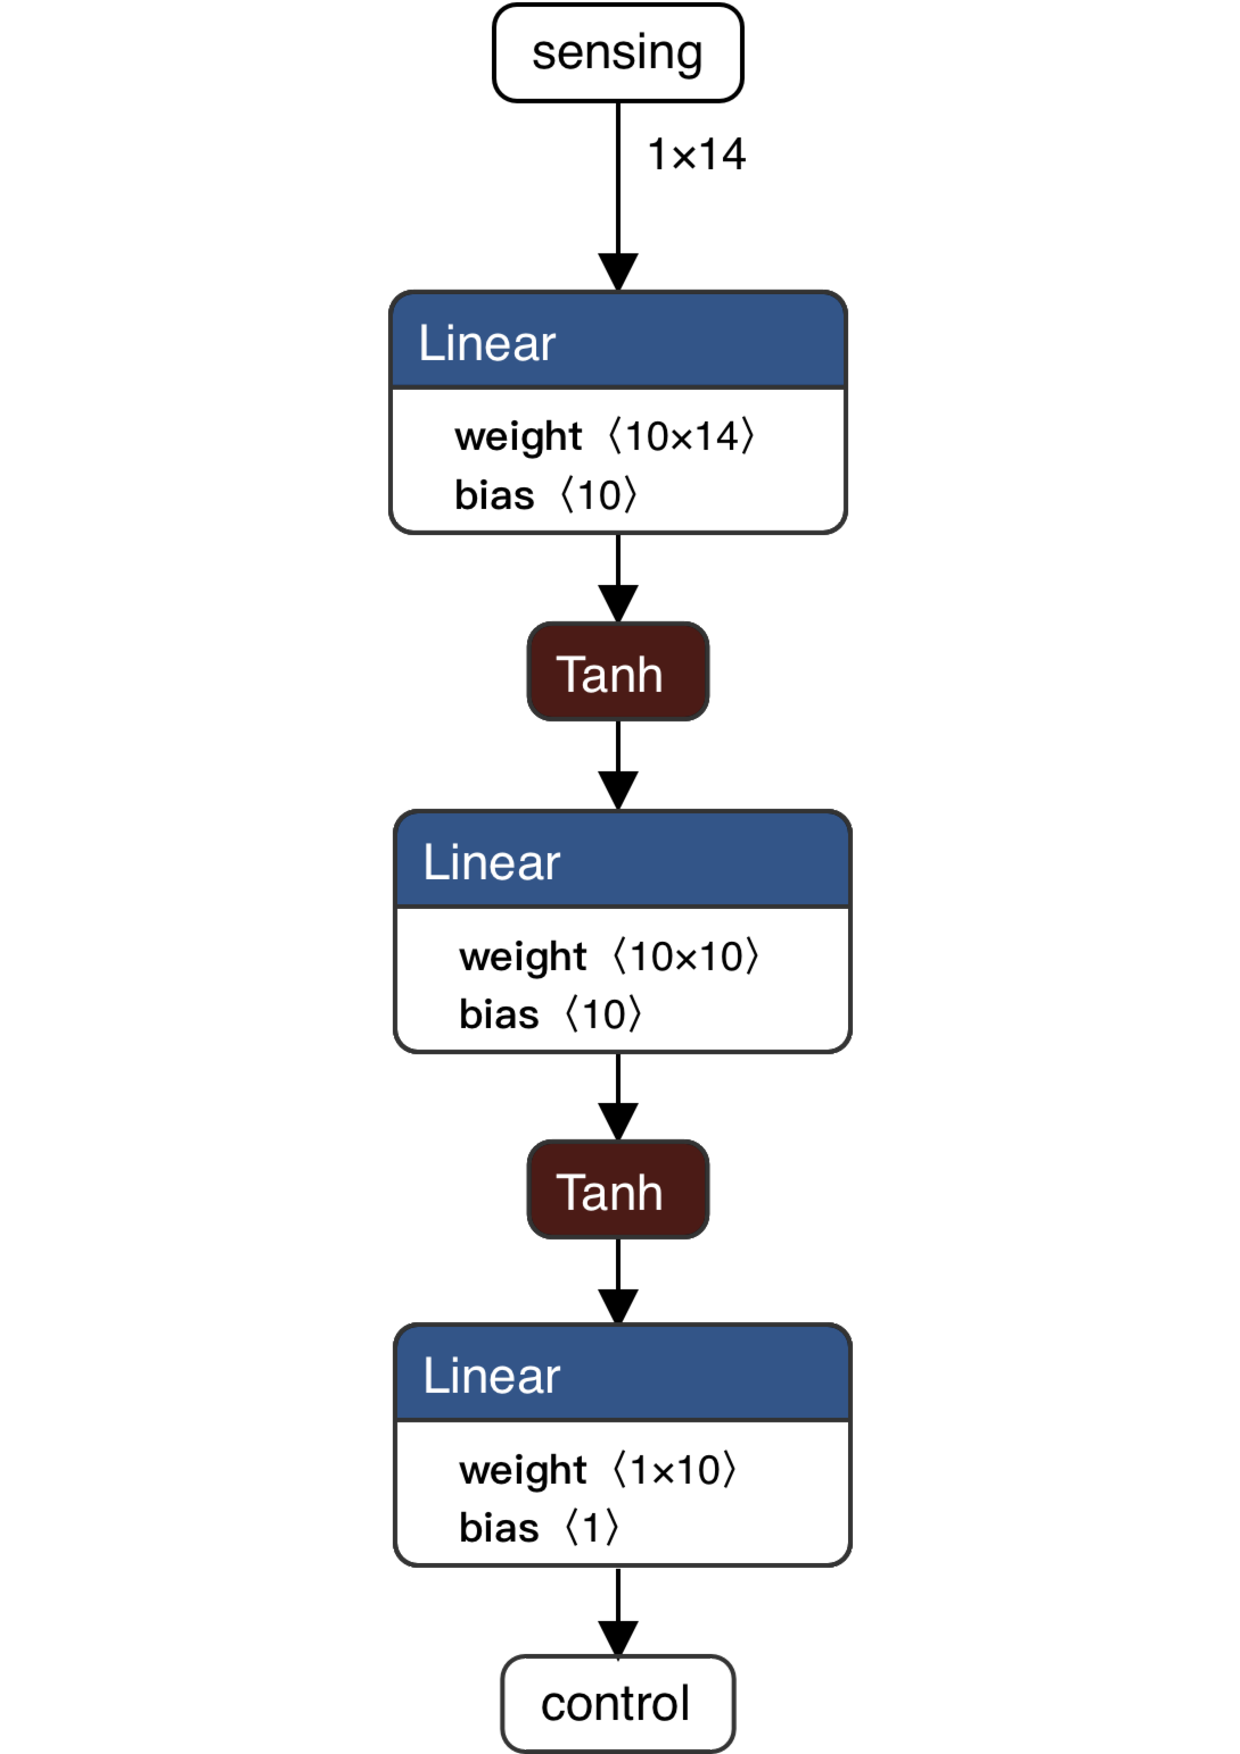
\includegraphics[width=.8\textwidth]{contents/images/task1distributed_all@4x}
		\caption{Network with $14$ input sensing.}
		\label{fig:singlenet-d14distributed1}
	\end{subfigure}
	\caption[Network architectures for the distributed approach.]{Visualisation of 
		the network architecture chosen for the distributed approach.}
	\label{fig:singlenetdistributed1}
\end{figure}

The Tanh non-linear activation function introduced in Section 
\ref{subsec:activationfun}, is applied to the first and second layer. 

As optimiser, we chose Adam, introduced in Section \ref{subsec:optimiser}, 
implemented in the \texttt{torch.optim} package, with a learning rate of $0.01$. 

Instead of performing gradient descent on the entire dataset, the training set is 
split in mini-batches of size $100$. In this way, an approximation of the gradient 
is produced, which makes the algorithm faster and at the same time, for 
sufficiently large batches, the result is indistinguishable.
Gradient descent algorithms are susceptible to ``getting stuck'' in local minima.
Mini-batches shuffle facilitate to avoid this problem by enabling the gradient to 
``bounce'' out of eventual local minimum, making it more variable by exploiting 
randomness, thereby helping convergence \cite[][]{meng2019convergence}.

All the models are trained for $50$ epochs and evaluated using the \gls{mse} loss 
function, defined in Section \ref{subsec:lossfunctions}, implemented in the 
\texttt{torch.nn} package.

\subsubsection{Task 1: Distributing the robots in space using communication}
\label{subsubsec:task1comm}

An alternative to the previous approach involves training a distributed network 
that also exploits a communication protocol between agents to decide the output 
control more reliably. 
Thus, using the same data collected before, we build a model that at each time 
step takes as input an array containing the response values of the sensors for each 
robot – \texttt{prox\_values}, \texttt{prox\_comm} or \texttt{all\_sensors} – and 
the messages received in the previous time step, communicated by the nearest 
agents (on the left and on the right), and produces 2 floats as output: the control, 
which is the speed of the wheels as before, and the communication, i.e. the 
message transmitted by the robot to its two neighbouring agents.

Even for this purpose, the model is independent of the number of agents in 
the simulations. Instead, now it is important to keep track of the time steps order 
since the input of the network requires the communication received which 
corresponds to the messages transmitted in the previous time step. To do so, 
preprocessing is applied to the dataset to combine consecutive 
time steps into a set of sequences. Therefore, we divide each simulation in 
sequences of length $2$, composed of two successive observations for each 
robot, using a stride of $1$.   
Accordingly, the shape of the model input has been transformed from $1 \times 
\mathtt{input\_size}$ to $\mathtt{seq\_length} \times \mathtt{N} \times 
\mathtt{input\_size}$, where \texttt{seq\_length} is fixed at $2$, $N$ is variable 
and \texttt{input\_size} can be $7$ or $14$.

\begin{figure}[!htb]
	\centering
	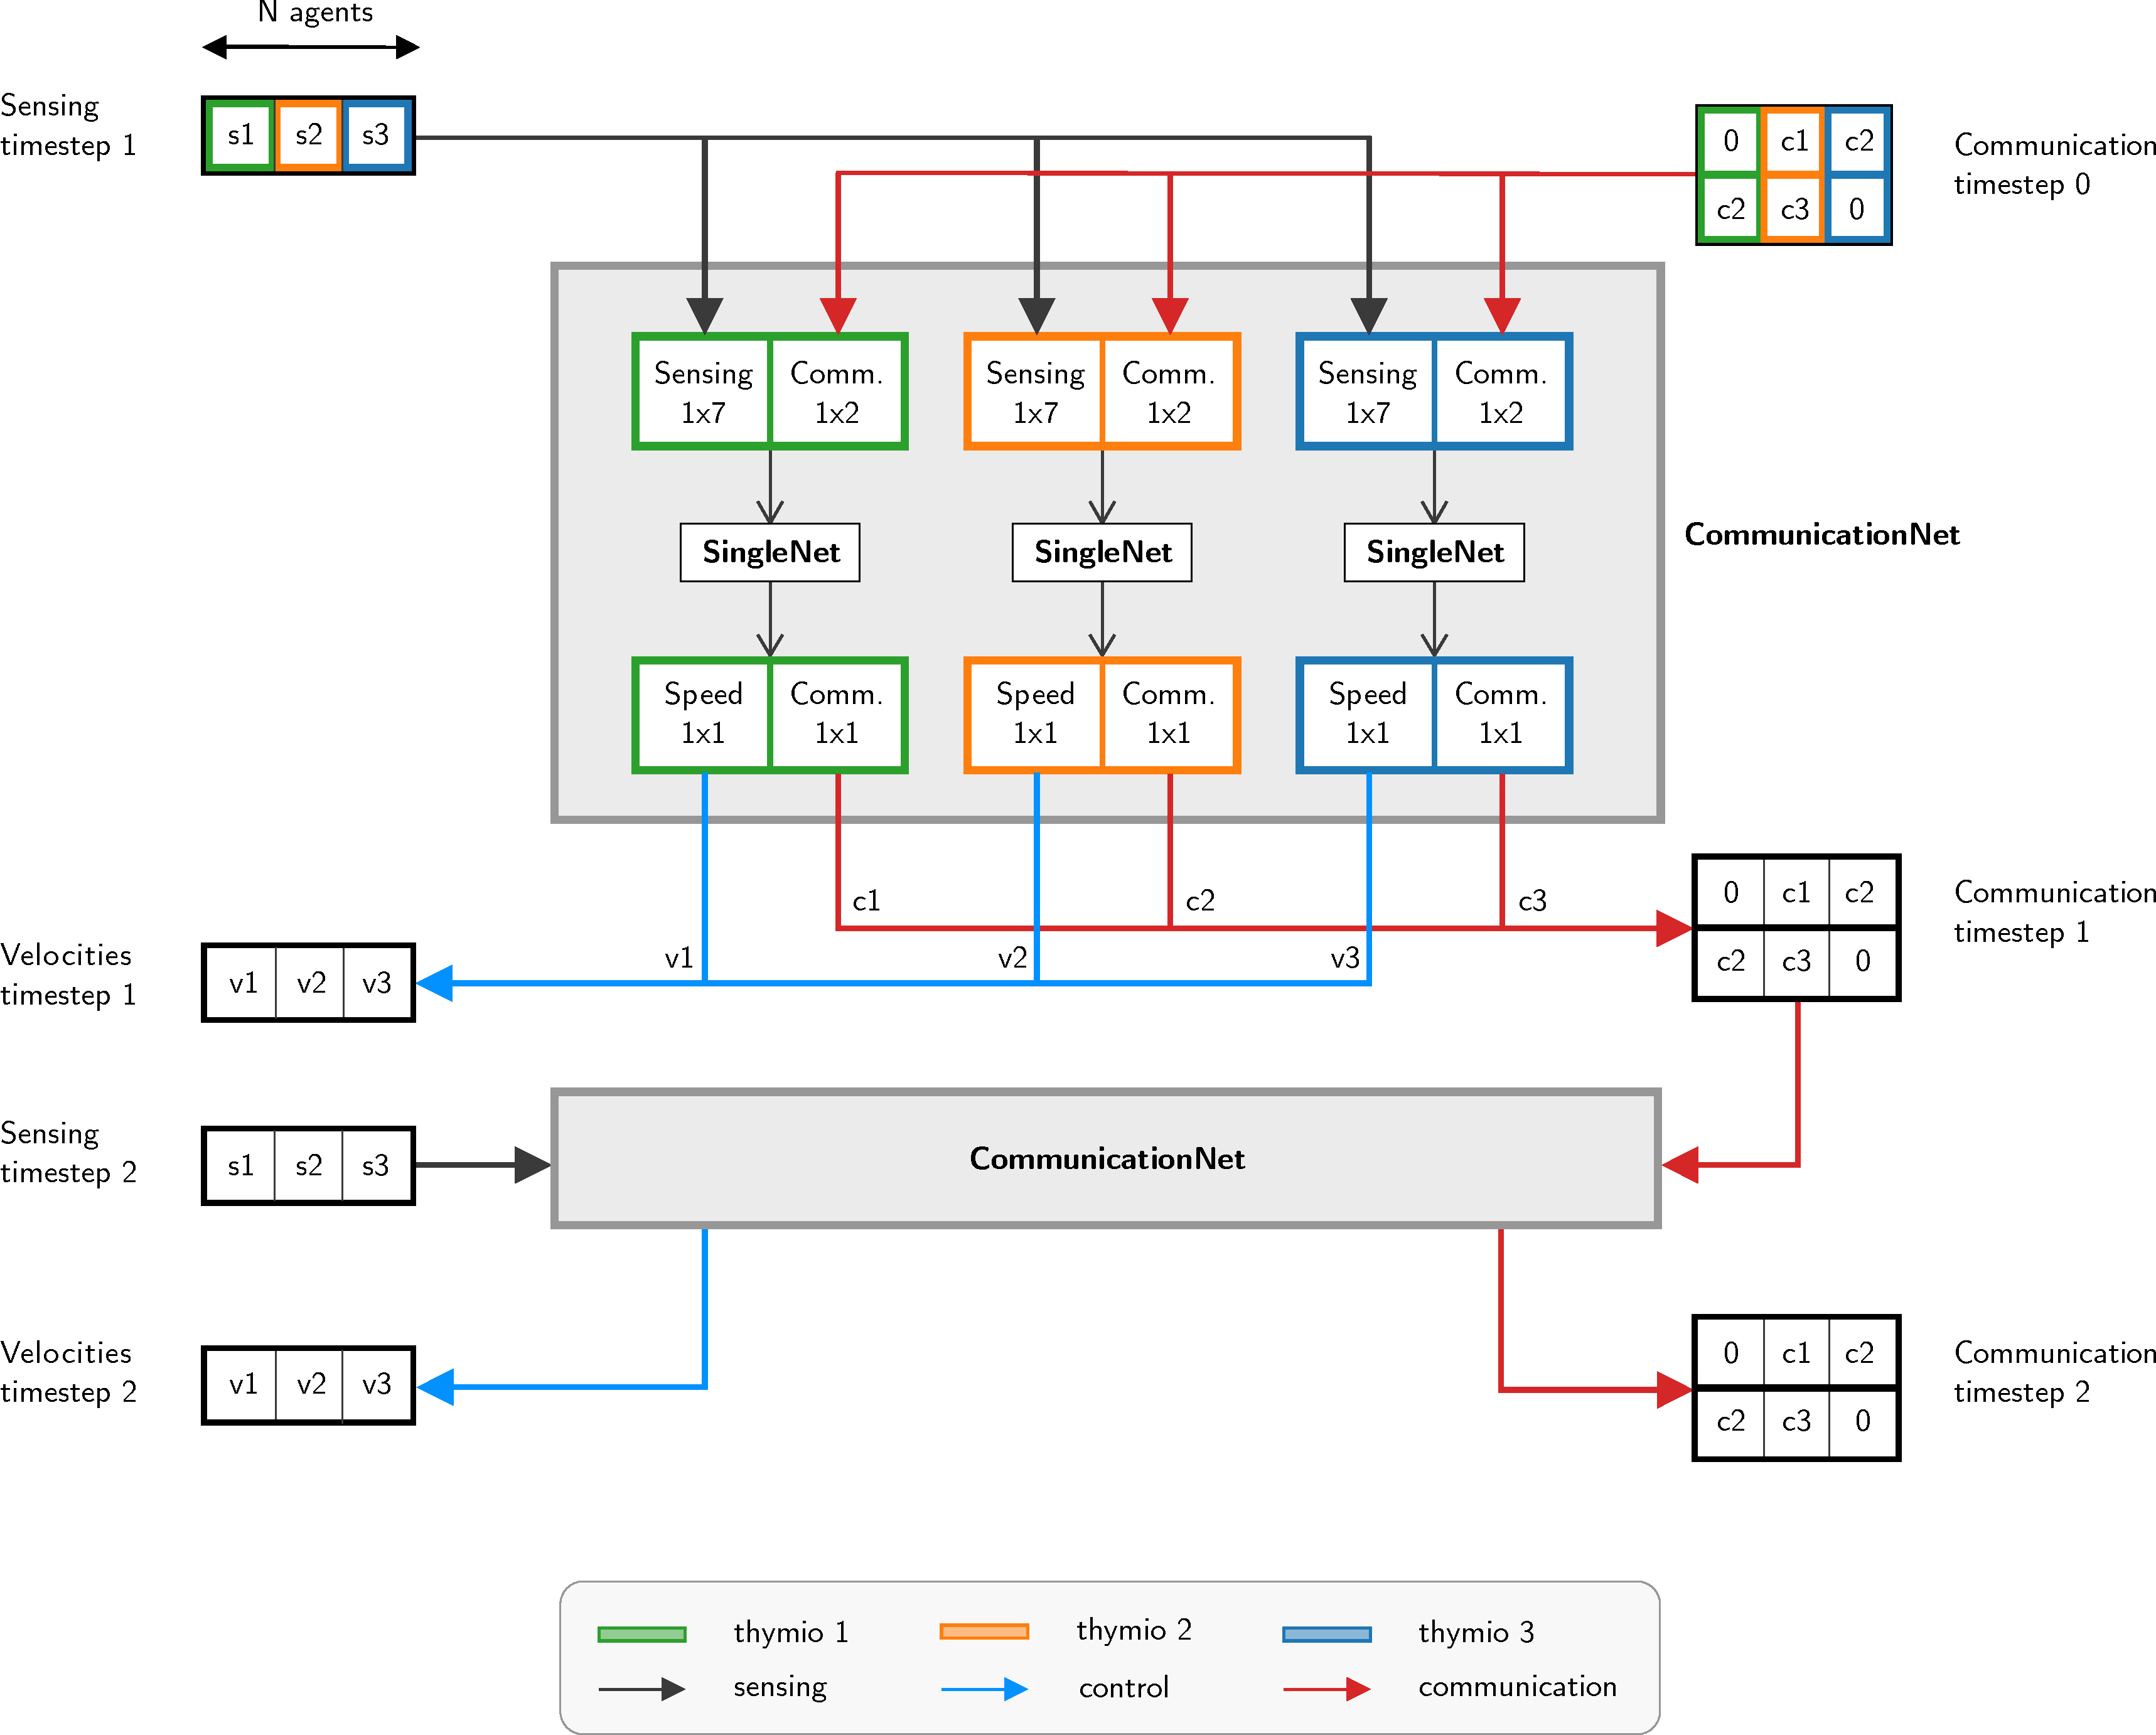
\includegraphics[width=\textwidth]{contents/images/commnet2}
	\caption[Communication network.]{Visualisation of the forward pass of the 
		communication network with three agents and a sequence composed by two 
		time steps.}
	\label{fig:commnet1}
\end{figure}

It is important to notice that the communication is not in the input since it is not 
contained in the original dataset, instead is treated as a hidden variable to be 
inferred. 
At the beginning of each sequence, there are no previous time steps to consider 
since no messages have been received yet. Therefore, a placeholder is randomly 
initialised, filled with float values in the range $[0, 1]$. 
The size of this array corresponds to the number of agents plus two elements, one 
at the beginning and one at the end of the vector, always set to $0$ since they are 
used to store the fact that the two extreme robots never receive messages 
respectively from the left or from the right. 
The random initialisation of this vector is essential to increase the generalization 
capabilities of the network during its training, showing it different starting 
situations.

As a consequence, we define a recurrent structure of the communication 
network, shown in Figure \ref{fig:commnet1}.
It is composed by two nested modules: in the outer level operates the 
\texttt{CommNet} that handles the sensing of all the agents, while in the inner the 
\texttt{SingleNet} that works on the sensing and the communication received by a 
single agent in a certain time step, producing as output the control and the 
communication to transmit. 
Therefore, this corresponds to a static unroll of a \gls{rnn}.%FIXME \cite[][]{}.

The architecture of the \texttt{SingleNet}, displayed in Figure 
\ref{fig:singlenetcomm1}, is almost the same as the one of the distributed 
model without communication: there are three linear layers each of size 
$\langle\mathtt{input\_size}, 10\rangle$,  $\langle 10, 10\rangle$ and $\langle 
10, 2\rangle$, where \texttt{input\_size} is the sum of the shape of the sensing 
and the two communication values received, one from the left and one from the 
right.

\begin{figure}[!htb]
	\centering
	\begin{subfigure}[h]{0.495\textwidth}
		\centering
		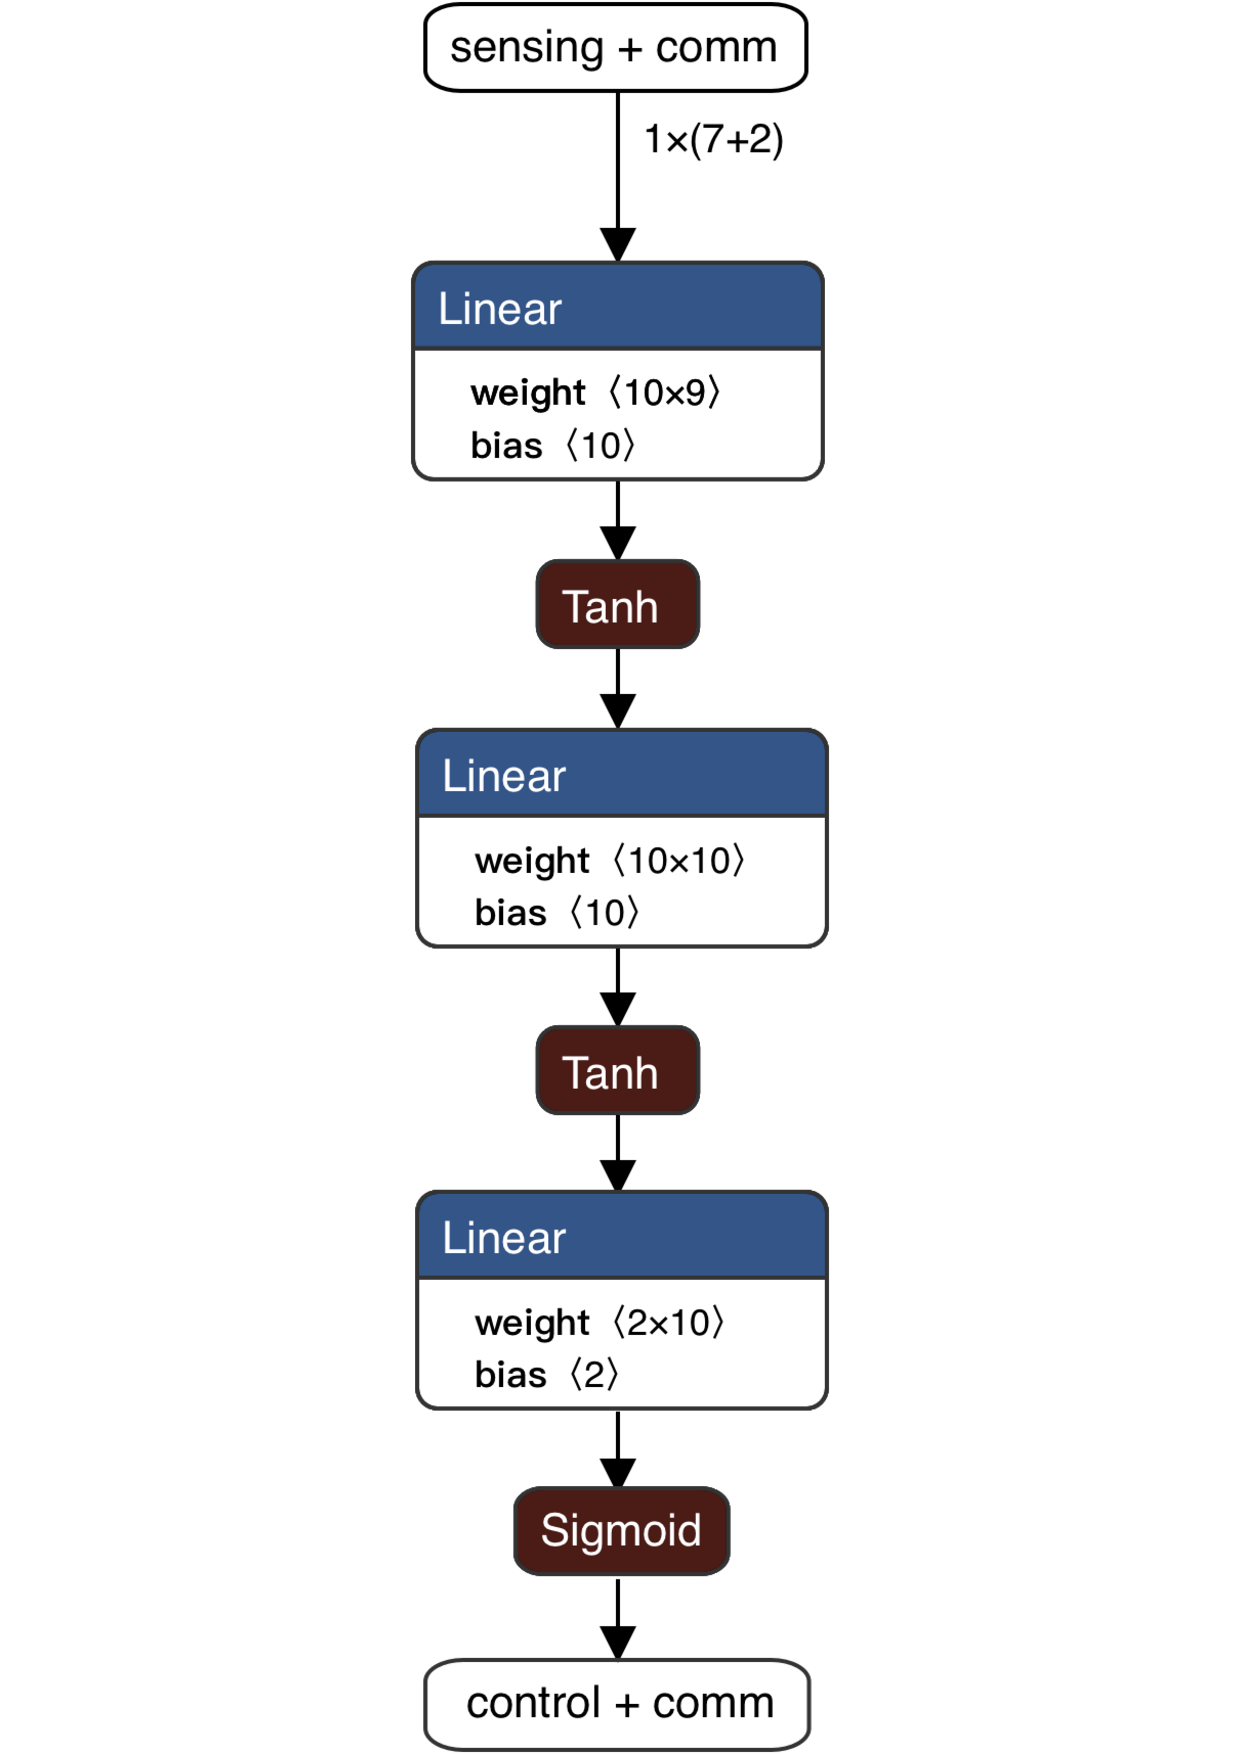
\includegraphics[width=.8\textwidth]{contents/images/task1distributedcomm@4x}%
		\caption{\texttt{SingleNet} with $7$ input sensing.}
	\end{subfigure}
	\hfill
	\begin{subfigure}[h]{0.495\textwidth}
		\centering
		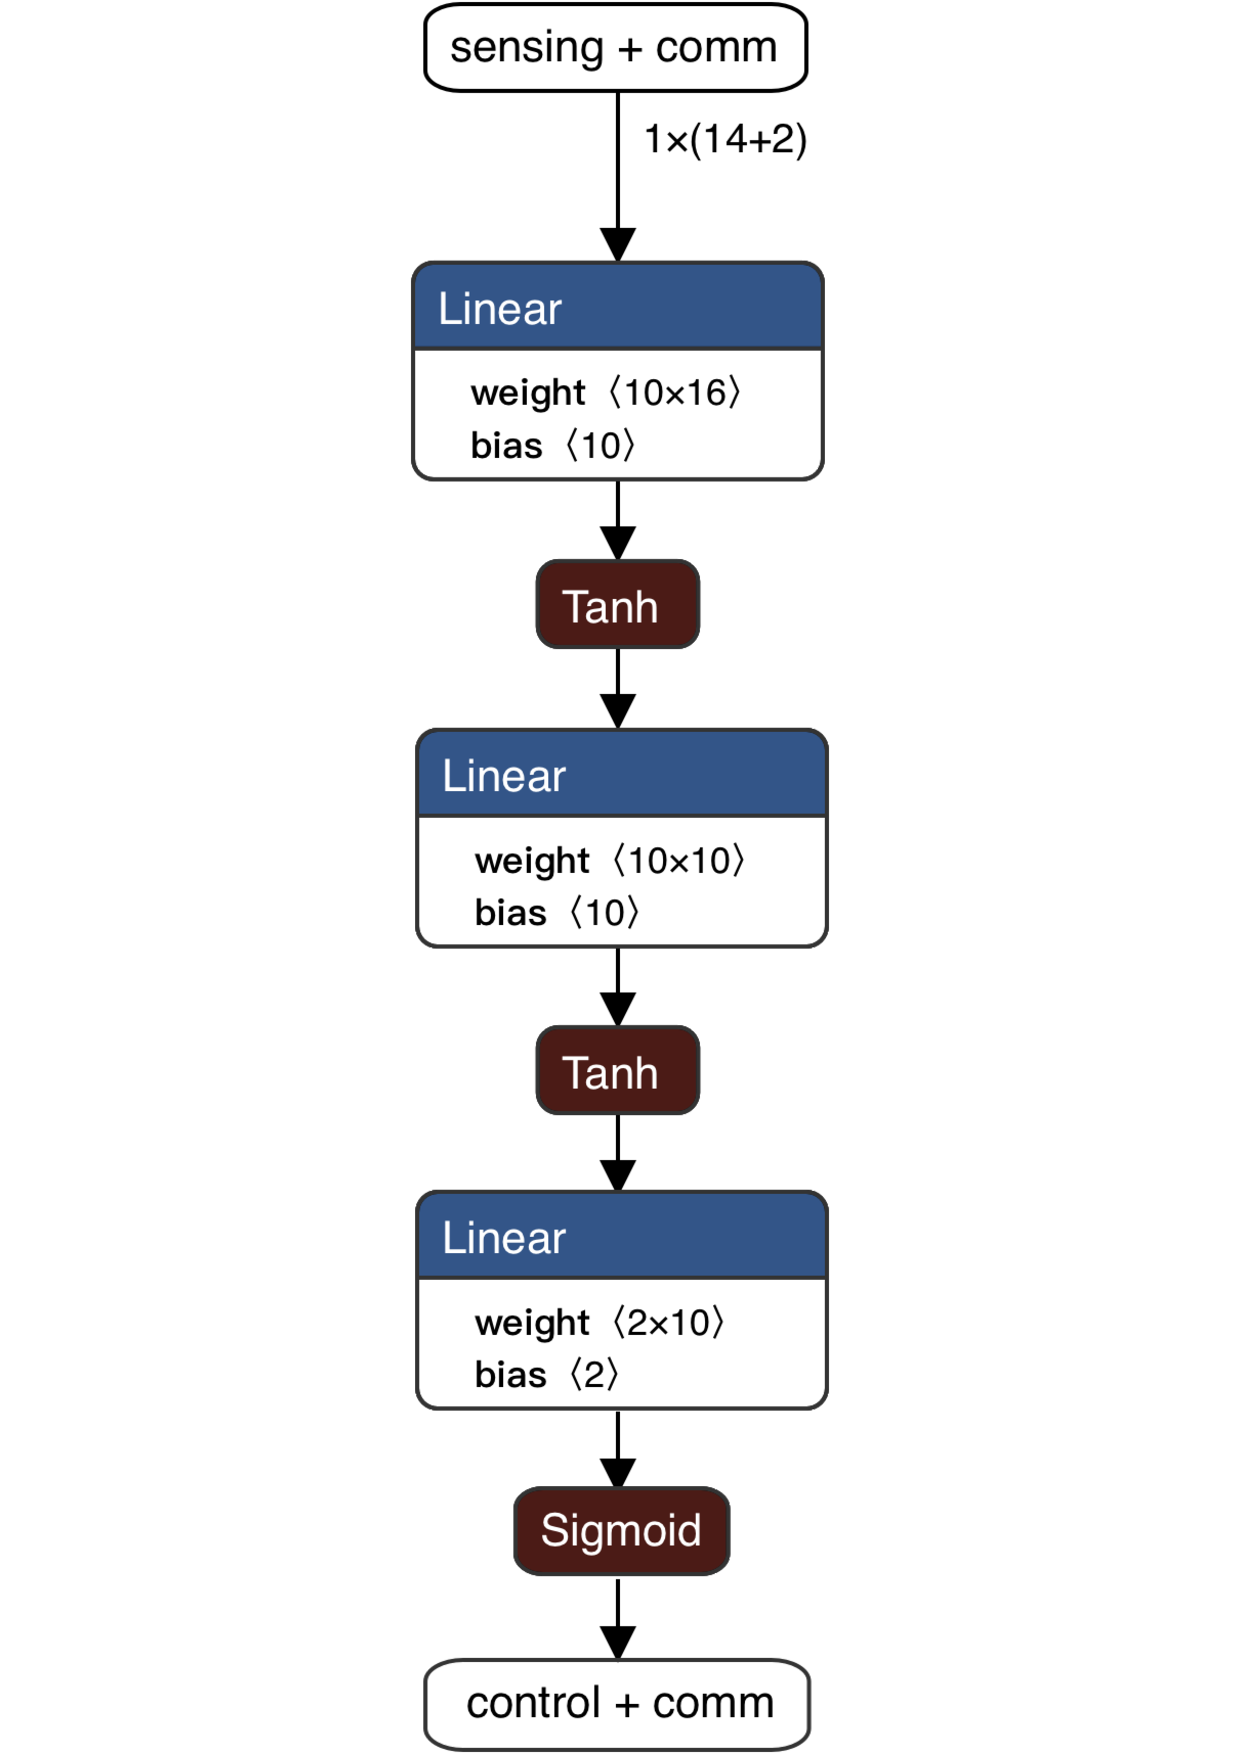
\includegraphics[width=.8\textwidth]{contents/images/task1distributed_allcomm@4x}
		\caption{\texttt{SingleNet} with $14$ input sensing.}
	\end{subfigure}
	\caption[Network architectures for the distributed approach with 
	communication.]{Visualisation of the network architecture chosen for the 
		distributed approach with communication in case of 7 or 14 inputs.}
	\label{fig:singlenetcomm1}
\end{figure}

As before, a Tanh non-linear activation function is applied to the first and second 
layer, while a sigmoid, introduced in Section \ref{subsec:activationfun}, is applied 
to the second dimension of the output in order to normalise it in the range $[0, 
1]$.

As before, we use Adam optimiser, addressed in Section \ref{subsec:optimiser}, 
but with a smaller learning rate, $0.001$. 
We split the dataset in mini-batches, this time of size $10$ and then we train 
the models for $500$ epochs. 
Finally, we evaluate the goodness of the predicted control using the \gls{mse} 
loss function, while the communication has to be inferred by the network.
Since the network is fully connected, the communication affects directly the 
output, and consequently, the error minimised. Improving the loss has an impact 
also on the communication latent variable, since the error is propagated through 
%FIXME
the internal network, in order to update the weight during the back-propagation 
step.

\subsubsection{Task 2: Colouring the robots in space}
In this scenario, it is possible to implement a network very similar to the one used 
for the previous task, that is the distributed approach with communication, 
described in Paragraph \ref{subsubsec:task1comm}, but this time ignoring the 
sensors readings.
Thus, using the same data collected before we build a model that at each time 
step takes as input for each robot only the messages received in the previous time 
step, communicated by the nearest agents (on the left and on the right), and 
produces as output an array of 2 floats, the first one is the probability of the agent 
top \gls{led} to be blue and the second is the communication, i.e. the message to 
be transmitted by the robot.

The communication network, whose structure is shown in Figure 
\ref{fig:commnet2}, is composed by two nested modules: in the outer-level 
operates the \texttt{CommNet} that handle the sensing of all the agents, while in 
the inner-level the \texttt{SingleNet} that works on the communication received 
by a single agent in a certain time step, producing as output the colour and the 
communication to transmit. 
\begin{figure}[H]
	\centering
	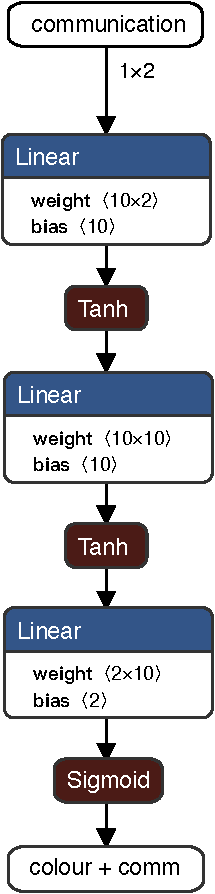
\includegraphics[width=.14\textwidth]{contents/images/task2allcomm}
	\caption[Network architectures for the communication approach.]{Visualisation 
		of the network architecture chosen for the 
		communication approach.}
	\label{fig:singlenetcomm2}
\end{figure}

The \texttt{SingleNet}, displayed in Figure \ref{fig:singlenetcomm2}, is composed 
by three linear layers of size $\langle \mathtt{input\_size}, 10\rangle$,  $\langle 
10, 10\rangle$ and $\langle 10, 2\rangle$, where \texttt{input\_size} 
corresponds to the two communication values received, one from the left and one 
from the right.

\begin{figure}[!htb]
	\centering
	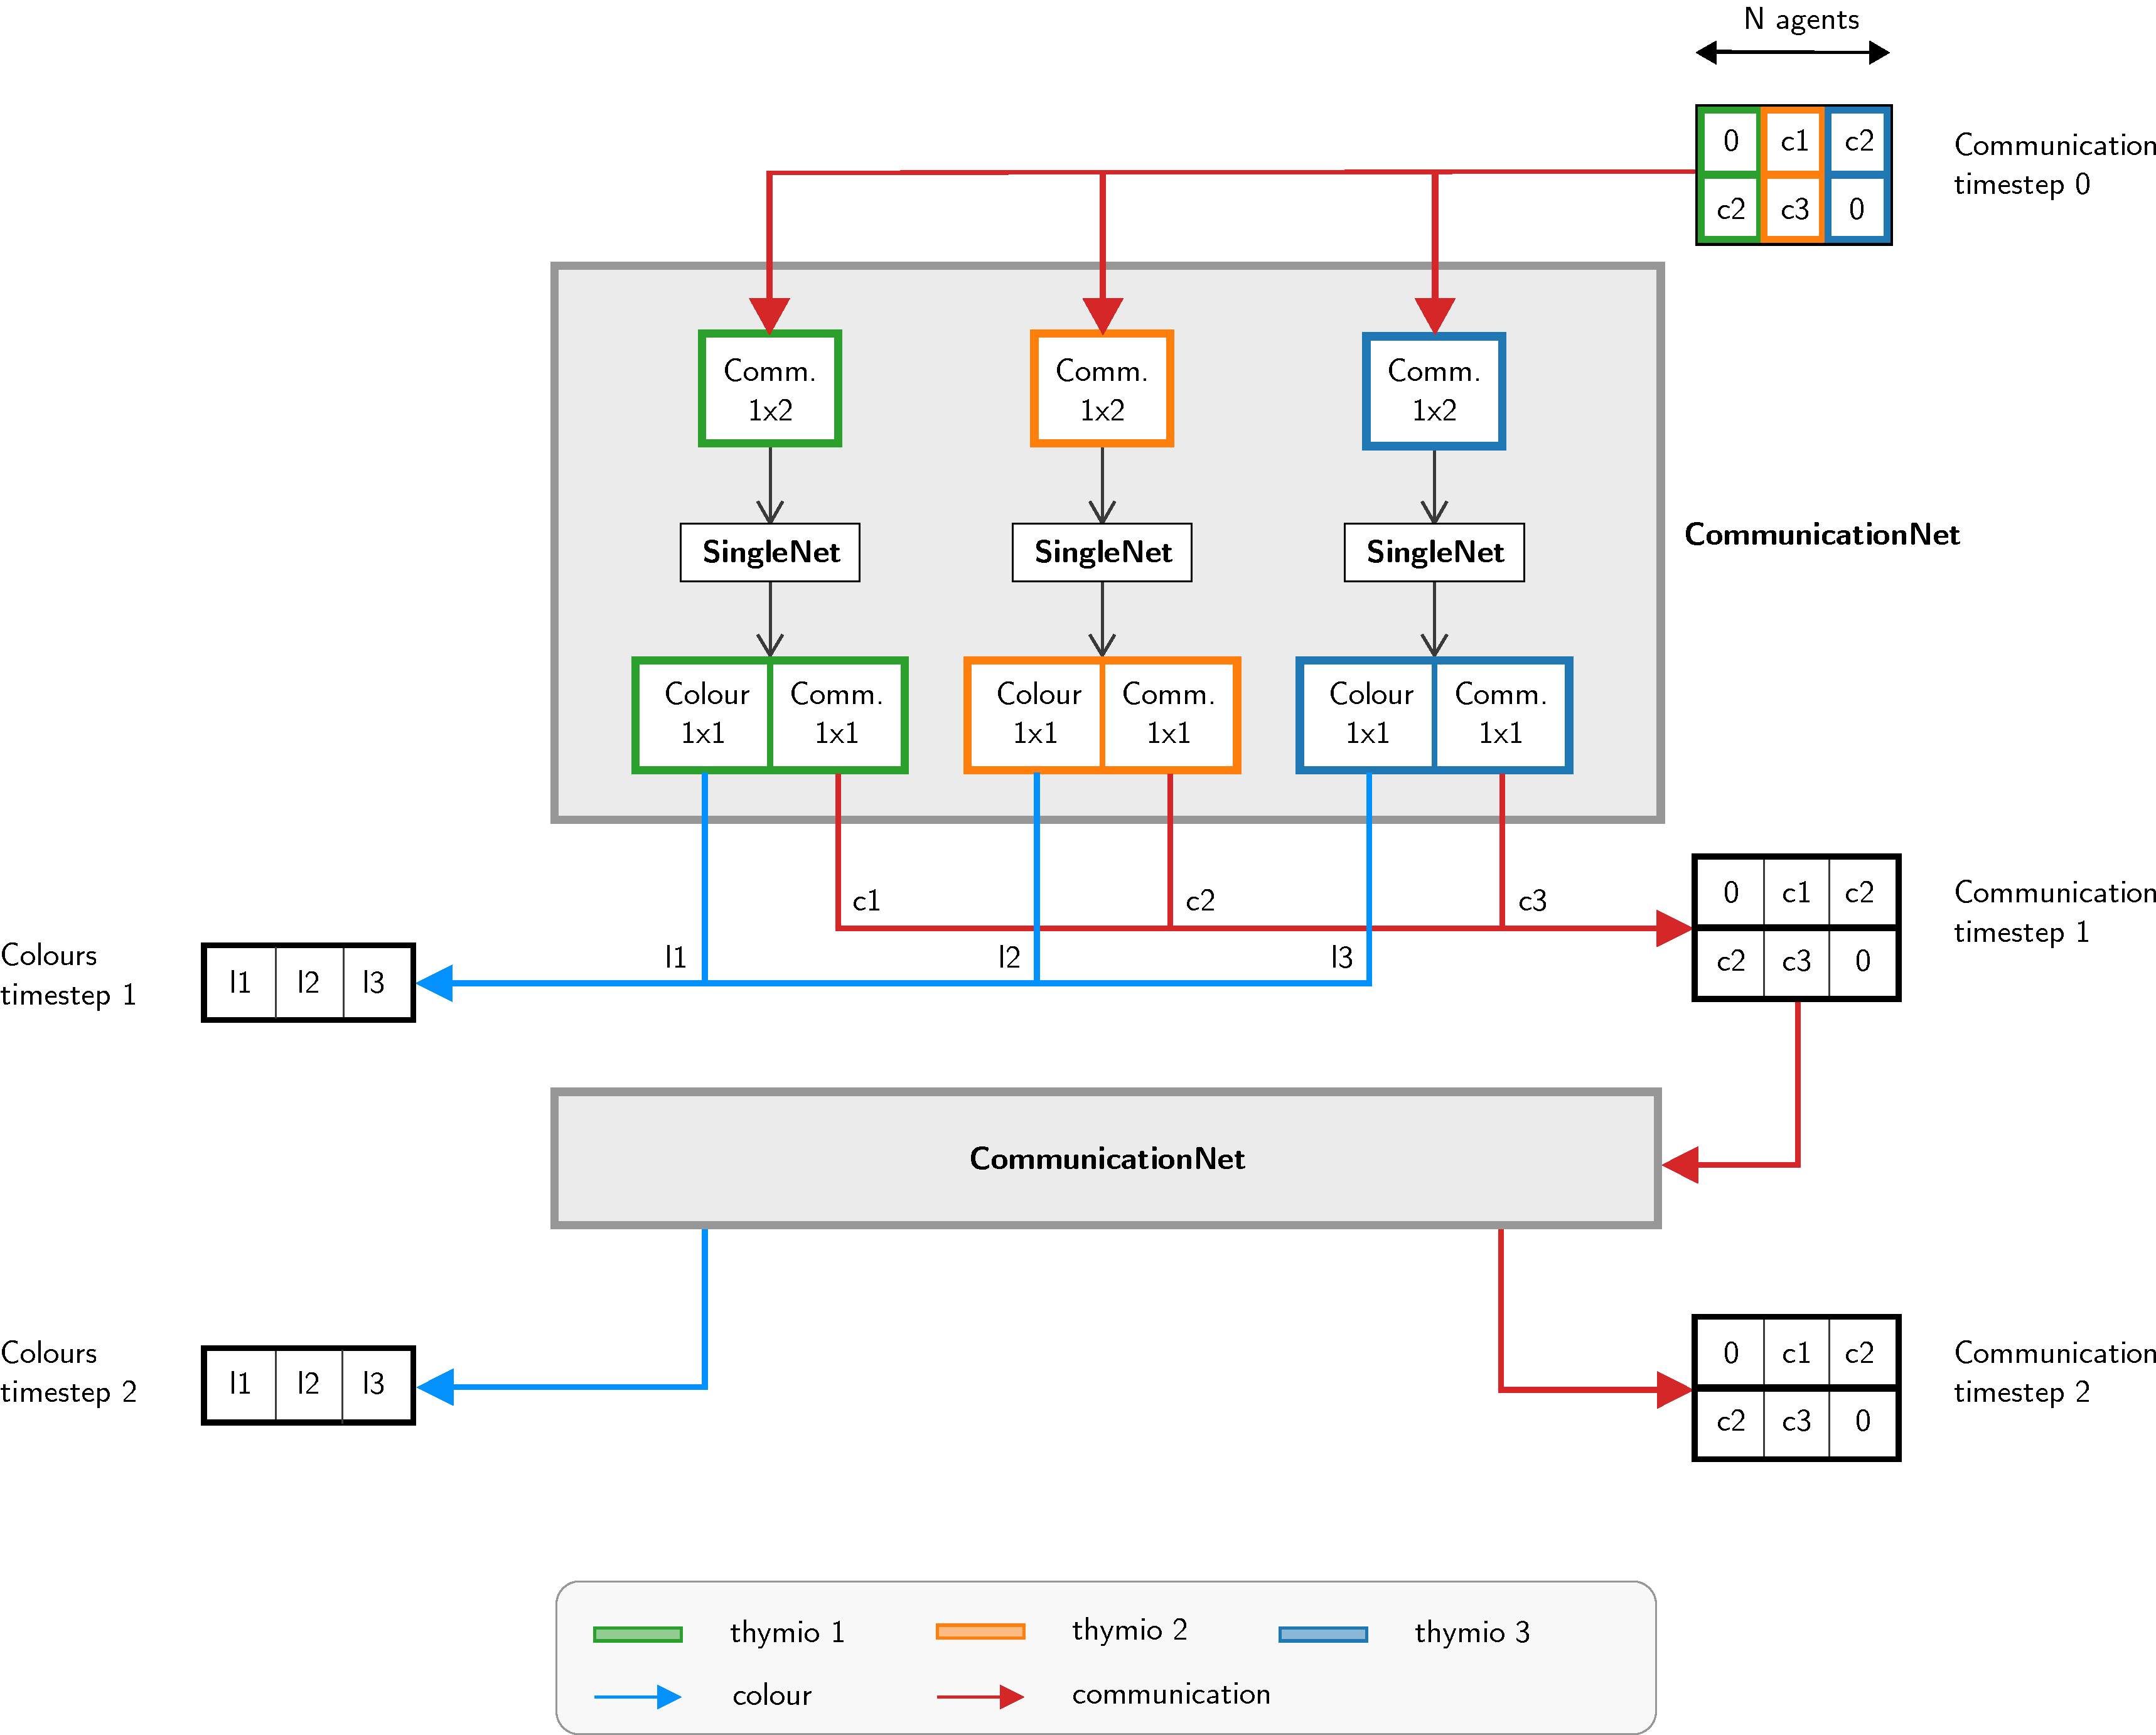
\includegraphics[width=\textwidth]{contents/images/commnettask2}
	\caption[Communication network of the second task.]{Visualisation of the 
		forward pass of the communication network with three agents and a 
		sequence 
		composed by two time steps.}
	\label{fig:commnet2}
\end{figure}

The activation functions used for this purpose are two, and are introduced in 
Section \ref{subsec:activationfun}.
To the first and second layer is applied a Tanh non-linear activation function, 
while a sigmoid to the output, in order to normalise it in the range $[0, 1]$.

As before, we use Adam optimiser but with a smaller learning rate, $0.001$. 
We split the dataset in mini-batches of size $10$ and then we train the models for 
$100$ epochs. 

In order to decide the metric to evaluate the goodness of the prediction, it is 
necessary to analyse the output of the network. As we said, the model returns, in 
addition to the communication, the colour that is actually the probability of the 
agent top \gls{led} to be blue. This means that, when the network produces a 0, 
the probability that the \gls{led} is blue is equal to 0, i.e. it is red; in the same way, 
1 means that instead, this will be blue. In this way, we define a simple policy 
function that returns the colour blue when the probability is between 0.5 and 1, 
and red otherwise, or when the probability is less than 0.5.
For this reason, instead of using the \gls{mse} loss function, as this is a binary 
classification problem we choose the \gls{bce}, defined in Section 
\ref{subsec:lossfunctions}, implemented in the \texttt{torch.nn} package.
It is important to remember that communication is still inferred as a latent 
variable.
